\section{Background}
\label{sec:background}

% PAGE TARGET: ~6 pages.
% Narrative organisation modelled on Andrew Liang 2024 chapter 1.
% Subsections: Motivation / Current Feature Extraction Techniques /
% Paper Imaging using DRM / Manuscript Dataset / Pipeline Overview.

\subsection{Motivation}
\label{sec:bg:motivation}

The process of making handmade paper in late medieval
and early modern Europe is as follows: a vatman dips a mould made of a wooden frame
with metal wires in between into a vat of 
fibre solution, lifts it out, and lets the water drain through the
frame's mesh~\cite[ch.~1]{darold2020paper}. The mould carries two sets
of perpendicular wires. A small number of stout chain wires, typically
spaced 2 to 3 centimetres apart, run from one short edge to the
other and provide structural support for other wires. On top of them, a much denser
layer of fine laid wires, of the order of 8 to 15 per
centimetre, runs perpendicular to the chain wires. As the wet fibre pulp
settles, it deposits more paper material in the spaces between wires than
above the wires, so that the dried paper sheet ends up
with a periodic thickness pattern that corresponds to the wire
layout~\cite{enomae2010laidlines}. Under intensive illumination, this
pattern appears as a series of pale and dark lines that is visible
to human eyes.

\begin{figure}[!htbp]
  \centering
  
\includegraphics[width=0.78\linewidth]{folio_anatomy}
  \caption{Reflected-light close-up of a folio from the present DRP
  benchmark (dataset 4, $\theta=15^\circ$ grazing illumination from
  $\phi=0^\circ$). The vertical, close-spaced banding visible across the
  field is the periodic thickness modulation cast by the laid wires of
  the mould; the wider feature at lower right is a diagonal artefact
  of the folio surface. Chain lines are spaced two to three centimetres
  apart and are not resolved at this magnification.}
  \label{fig:bg:folio_anatomy}
\end{figure}

Each mould was made by hand, with wires drawn and tied by an individual
artisan, so no two moulds are exactly identical. Moreover, paper was
almost always made in pairs: two near-identical moulds were used in
alternation by the same artisan to keep production continuous while
each sheet was being dried. The result is that, every batch of paper
from a given workshop carries a recognisable signature in
the geometry of its laid and chain lines~\cite[ch.~2]{darold2020paper},
aside from the watermark that today mainly contributes to the recognition and 
sourcing of medieval papers.
Codicologists utilise this signature together with watermarks to group folios that come from the
same mould or mould pair, and from there to assign manuscripts to a
region, a workshop, or even a specific year.

To this day, the analysis of laid line features is still largely
manual. A researcher inspects each folio under raking or transmitted
light, counts wires with assistance of a short ruler, and records a single density
figure in lines per centimetre. The procedure is slow,
observer dependent, and exposes fragile paper manuscripts to repeated
handling. It also discards almost all of the information present in
the original image, including the variation of density across the page, the
local orientation of the laid lines, and the distribution of wire
diameters; instead, all information is collapsed to a single scalar. At the same time,
major research libraries including Cambridge University Library,
the Bodleian, and the Bibliothèque nationale de France, now
 capture multispectral image stacks of their
holdings~\cite{miniare} as a basis. These stacks contain far more
information than a single density estimate, but no robust automated
pipeline yet exists to turn them into quantitative
 data as a mould fingerprint that codicology actually requires. Closing
that gap is the central aim of this project.

\subsection{Current Feature Extraction Techniques}
\label{sec:bg:prior_extraction}

The idea of automated extraction of laid and chain lines from digital images of
historical paper has a small but established literature. Most existing
techniques operate on transmitted light or radiographic images,
treating the folio as a two-dimensional signal with a dominant spatial
frequency. The earliest systematic study, by Hiary and
Ng~\cite{hiary2007paper}, applied projection-based Fourier methods to
 transmitted light scans, extracting the laid line density
from the dominant peak in a one-dimensional power spectrum of the
column sum. Subsequent variants included Gabor filter banks,
autocorrelation, or wavelet decompositions, of which the AD751
software of Atanasiu~\cite{atanasiu_ad751} is a widely used
implementation. These methods are simple to implement and reasonably
robust to global illumination, but they share three common weaknesses:
the line orientation must be supplied externally or estimated as a
separate pre-processing step, the spectrum is computed over the whole
image and therefore averages out local variations from curvature or
ink coverage, and no uncertainty figure accompanies the extracted
density.

A second branch of work has grown out of large scale bibliographic
projects such as the Bernstein and WIES
initiatives~\cite{wenger2010bernstein,wies}, which catalogue watermarks
across European collections. The emphasis there was to capture
high quality transmitted light images and to build searchable
databases of watermark designs, with relatively little attention to
the chain line and laid line features that surround the watermark.
Pipelines in this branch tend to be tuned per image by a human
operator rather than run as a single automated process. Radiographic
methods such as the chain line detection of Van der
Lubbe~\cite{vanderlubbe2001rembrandt}, which combines morphological filters
with vertical projections, give cleaner signals but require imaging techniques
that are too expensive to implement for most institutions.

More recent work has approached the problem from two further
directions. Dedicated transmitted light imaging hardware such as
the Watermark Imaging System of Sethares et
al.~\cite{sethares2023wimsy} produces aligned surface, raking light
and transmitted light captures that make laid and chain features
easier to read, and deep learning segmentation models such as
ChainLineNet~\cite{sindel2021chainlinenet} can localise chain lines
in transmitted light scans with very little hand annotation.
A work closest to the present project is the moldmate-
identification system of Gorske et al.~\cite{gorske2021moldmate},
which combines watermark geometry, chain line spacing and laid line
density into a single quantitative match score; the present
pipeline addresses only the laid line component of that
combination, but as an automated detector with a per-folio
confidence figure.

The transmitted light and radiographic modalities used by these prior
methods share a more fundamental limitation: they collapse the
three-dimensional shape feature of the folio surface onto a single
two-dimensional intensity image. Such features could include subtle ridges and valleys on each side of the page left by the laid lines, and they
carry information that is invisible to flat imaging. The
following section describes the alternative imaging modality on which
this project is built.

\subsection{Paper Imaging using Directional Reflectance Microscopy}
\label{sec:bg:drm}

% --- DRM apparatus paragraph --
The data analysed in this report were acquired using a directional
reflectance microscope (DRM) developed by the AddME Lab in the
Department of Engineering at the University of Cambridge. The
instrument fixes a camera above a sample stage and steps a
controllable light source through a regular grid of elevation and
azimuth angles, capturing one image per direction. The original
purpose of the DRM was to characterise the surface texture of
crystalline metallic samples~\cite{gaskey2020opticalchar,
wittwer2021drm}, and its first application to handmade paper is
recent. Conceptually the DRM sits in the broader family of
reflectance transformation imaging (RTI) techniques introduced by
Malzbender et al.~\cite{malzbender2001ptm}, which record the
per-pixel reflectance as a function of illumination direction
rather than as a single value; the DRM differs from a
typical RTI capture in the density of the angular sampling lattice
and in the microscope-scale optical resolution.

\begin{figure}[!htbp]
  \centering
  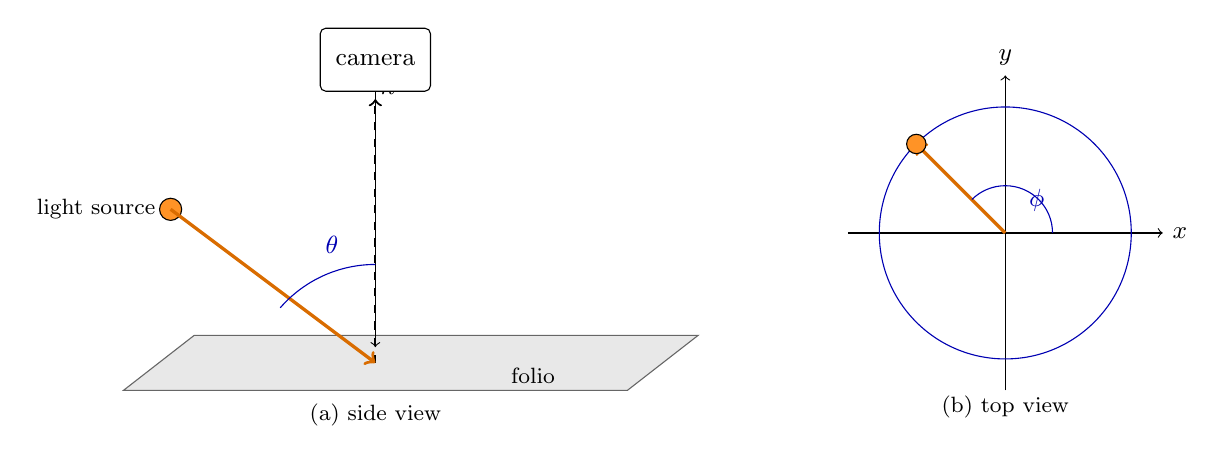
\begin{tikzpicture}[scale=1.0, every node/.style={font=\small}]
    % --- side view: theta angle ----------------------------------------
    \begin{scope}
      % Sample stage (the folio), drawn in perspective
      \draw[fill=gray!18, draw=black!60]
        (-3.2,0) -- (3.2,0) -- (4.1,0.7) -- (-2.3,0.7) -- cycle;
      \node[anchor=west] at (1.6,0.18) {\footnotesize folio};

      % Page normal
      \draw[->, thick, dashed] (0,0.35) -- (0,3.7)
        node[above right=-2pt] {$\hat{n}$};

      % Camera box, fixed on the normal
      \node[draw, rounded corners=2pt, minimum width=1.4cm,
            minimum height=0.8cm, fill=white] (cam) at (0,4.2) {camera};
      \draw[->] (cam.south) -- (0,0.55);

      % Light source at elevation theta from the normal
      \coordinate (src) at (-2.6,2.3);
      \filldraw[fill=orange!85, draw=black] (src) circle (4pt);
      \node[left=2pt] at (src) {\footnotesize light source};
      \draw[->, very thick, orange!85!black] (src) -- (0,0.35);

      % Theta arc
      \draw[blue!70!black] (0,1.6) arc[start angle=90, end angle=139, radius=1.6];
      \node[blue!70!black] at (-0.55,1.85) {$\theta$};

      \node[anchor=north] at (0,-0.05) {\footnotesize (a) side view};
    \end{scope}

    % --- top view: phi azimuth -----------------------------------------
    \begin{scope}[xshift=8cm, yshift=2cm]
      \draw[->] (-2,0) -- (2,0) node[right] {$x$};
      \draw[->] (0,-2) -- (0,2) node[above] {$y$};
      \draw[blue!70!black] (0,0) circle (1.6);
      % Projected source direction at phi
      \draw[->, very thick, orange!85!black] (0,0) -- (-1.13,1.13);
      \filldraw[fill=orange!85, draw=black] (-1.13,1.13) circle (3.5pt);
      \draw[blue!70!black] (0.6,0) arc[start angle=0, end angle=135, radius=0.6];
      \node[blue!70!black] at (0.4,0.42) {$\phi$};
      \node[anchor=north] at (0,-1.95) {\footnotesize (b) top view};
    \end{scope}
  \end{tikzpicture}
  \caption{Schematic of the directional reflectance microscope. The
  camera is fixed normal to a flat sample stage that carries the folio,
  and a programmable light source is stepped through a regular grid in
  elevation $\theta$ (from the page normal $\hat n$) and azimuth $\phi$
  (in the plane of the page). For each grid point a single frame is
  captured; the stack of all frames is the directional reflectance
  profile (DRP) used throughout this report.}
  \label{fig:bg:drm_schematic}
\end{figure}

% --- DRP definition paragraph --
For each spatial pixel $(x, y)$ on the folio, the DRM produces a
sampled reflectance function $I(x, y; \theta, \phi)$ where $\theta$
is the elevation angle of the source measured from the page normal
and $\phi$ is its azimuth in the plane of the page. The full
collection of these pixel-wise functions across the image is called
the directional reflectance profile (DRP) stack. A DRP is visualised on a single pixel as an annular heat map: the outer
ring corresponds to grazing illumination, the inner ring to
near-normal illumination, and the angular coordinate around the
annulus maps to the source azimuth.

\begin{figure}[!htbp]
  \centering
  
\includegraphics[width=0.55\linewidth]{drp_polar}
  \caption{Annular DRP at a single pixel of the benchmark folio
  (dataset~4, $50 \times 50$ pixel average centred near mid-page,
  background-subtracted). Radial coordinate is the source elevation
  $\theta$ (ranging from $10^\circ$ to $65^\circ$); angular coordinate
  is the source azimuth $\phi$ (full circle, $9^\circ$ steps). The
  two-lobed brightness pattern at $\phi \approx 0^\circ$ and
  $\phi \approx 180^\circ$ is the signature of a laid-line shadow:
  the pixel is brightest when the wires are side-illuminated from
  either side along their common normal, and dimmest when the source
  azimuth is parallel to the wires.}
  \label{fig:bg:drp_polar}
\end{figure}

% --- Why DRP suits laid line detection paragraph --
The DRP is well suited to laid line analysis because the laid line
features of the paper surface are too subtle and shallow to read from a flat
image, but produce a clear directional signature in reflected light.
Under uniform illumination, the thickness variation
caused by the laid wires gives only weak greyscale contrast. Viewed
from a grazing angle aligned with the line normal, however, the same
modulation casts a strong, directional shadow that is easy to see.
A DRP records the full $(\theta, \phi)$ dependence of that shadow in
a single imaging, so a detector built on top of a DRP can find
the orientation and period at which the
laid line signal is strongest, without the extra need to supply these information externally. This property is what makes the
present pipeline simpler to operate than the projection based
methods of the previous section, where orientation has to be
supplied as an external parameter.

\subsection{Manuscript Dataset}
\label{sec:bg:dataset}

The folios analysed in \Cref{sec:benchmark} were drawn from the
Mapping Paper in Medieval England corpus curated by Professor
Orietta Da Rold and the Manuscripts Lab in the Faculty of English at
Cambridge~\cite{darold2020paper}. The corpus comprises 5841
manuscripts of which at least 736 are written on
paper~\cite{mappingpaper}; from these, nine folios
spanning four manuscript stocks were selected for the present
benchmark. The shelfmarks used in the report follow the Cambridge
University Library convention and are listed alongside the
spreadsheet ground truth density and the folio metric bundle
in \Cref{sec:benchmark:msi:perfolio}. Every folio in the benchmark
was additionally counted by hand using a custom annotation tool,
giving a ground truth that is set against both
the pipeline output and the catalogue spreadsheet in
\Cref{sec:benchmark:msi:manual_gt}.

\subsection{Pipeline Overview}
\label{sec:bg:contributions}

The work reported here treats the following inverse problem. Given
a DRP stack $I(x, y, \theta, \phi)$ together with the imaged
field-of-view width in centimetres, the pipeline must return three
quantities: the laid line density $\rho$ in lines per centimetre,
the local wire diameter $w$ expressed as a full-width-at-half-maximum
in millimetres, and the local laid line orientation $\alpha(x, y)$
in degrees, along with an associated uncertainty for each. The
pipeline must operate with no folio-specific parameter tuning beyond the
optical scale, and must report enough evidence for a codicologist
 to judge whether to trust each estimate.

The developed pipeline supports two different kinds of input
through a single common framework. The multi-phi DRP variant is
the original imaging methodology of the project and operates on the full
directional reflectance stack produced by the DRM instrument. It
aggregates normalised power spectra across all available
azimuthal views, recovers a single dominant period, and combines phases
of each view into a weighted circular mean with polarity and
half period autocorrections. The single image MSI variant is the
extension that lets the same pipeline run on the single-frame
transmitted light scans already held in major MSI archives: it
applies a radial fast Fourier transform followed by a single
Gabor cleanup pass at the locked period. Both variants share a
common preprocessing step (background subtraction, automatic
line direction detection by spectral power scan, polarity flag,
configurable period search band), and feed the same evaluation
bundle of quality metrics described in
\Cref{sec:multiphi:evaluation}. \Cref{fig:pipeline_diagram}
summarises the overall flow.

\begin{figure}[!htbp]
\centering
\begin{tikzpicture}[
  node distance=8mm and 5mm,
  every node/.style={font=\small},
  input/.style={rectangle, draw, minimum width=3.2cm, minimum height=0.7cm, fill=blue!8, align=center},
  process/.style={rectangle, draw, rounded corners, minimum width=4.6cm, minimum height=0.7cm, fill=orange!10, align=center},
  variant/.style={rectangle, draw, rounded corners, minimum width=5cm, minimum height=1.6cm, fill=orange!18, align=center},
  output/.style={rectangle, draw, minimum width=5cm, minimum height=0.8cm, fill=green!12, align=center},
  arr/.style={-Latex, thick}
]
\node[input] (drp) {DRP stack ($N$ grazing images)};
\node[input, right=1.2cm of drp] (msi) {Single MSI image};

\node[process, below=10mm of $(drp.south)!0.5!(msi.south)$] (bg) {Background subtraction};
\node[process, below=of bg] (autodir) {Automatic line-direction detection};
\node[process, below=of autodir] (pol) {Polarity flag + period search band};

\node[variant, below=10mm of pol, xshift=-3.4cm] (mp) {Multi-phi DRP variant\\\footnotesize aggregated spectra $\to$ period\\\footnotesize per-image phase fit with polarity\\\footnotesize correction; weighted circular mean};
\node[variant, below=10mm of pol, xshift=3.4cm] (si) {Single-image MSI variant\\\footnotesize radial FFT $\to$ period\\\footnotesize Gabor cleanup; phase fit\\\footnotesize at locked period};

\node[output, below=10mm of pol, yshift=-2.4cm] (out) {Density, wire FWHM, per-folio grid\\and 4-/5-metric evaluation bundle};

\draw[arr] (drp.south) -- ++(0,-3mm) -| (bg.north);
\draw[arr] (msi.south) -- ++(0,-3mm) -| (bg.north);
\draw[arr] (bg) -- (autodir);
\draw[arr] (autodir) -- (pol);
\draw[arr] (pol.south) -- ++(0,-3mm) -| (mp.north);
\draw[arr] (pol.south) -- ++(0,-3mm) -| (si.north);
\draw[arr] (mp.south) |- ([yshift=3mm]out.north) -- (out.north);
\draw[arr] (si.south) |- ([yshift=3mm]out.north) -- (out.north);
\end{tikzpicture}
\caption{Pipeline overview; two input modalities, common preprocessing, two detector variants, shared output.}
\label{fig:pipeline_diagram}
\end{figure}

There are three contributions of this project that deserve highlighting. The first
is the staged DRP-based pipeline itself, which to the author's
knowledge is the first automated pipeline to recover laid line
density, orientation and wire diameter from a DRP stack
without folio specific parameter tuning. The second is a synthetic
phantom characterisation framework that supports four orthogonal
sweeps (period, signal-to-noise ratio, orientation, and wire width)
over a controllable line pattern generator; this generator is used in
\Cref{sec:benchmark:msi:phantom} to map the failure modes of the
detector one variable at a time before applying it to real data.
The third is the nine folio benchmark introduced in
\Cref{sec:bg:dataset}, which together with the manual ground truth
on those folios provides strong quantitative accuracy figures
yet reported for an automated laid line pipeline on real manuscript
material.

Subsequent to this section, \Cref{sec:first_attempts} describes
two earlier detection attempts that did not work
well, both because they shaped the design of the final pipeline
and because the comparison with those pipelines form the natural
ablation baseline. \Cref{sec:multiphi} describes the detection
chapter itself, including the common preprocessing framework, the
single image MSI variant, the multi-phi DRP variant, and the
shared evaluation metric bundle. \Cref{sec:benchmark} presents
the synthetic phantom characterisation, the nine folio MSI
benchmark, the manual ground truth comparison, the four
 DRP datasets including both real manuscripts and controlled reproduction paper
reproduction, and a catalogue of failure modes. \Cref{sec:discussion}
interprets these results and addresses the limitations of the present
pipeline. \Cref{sec:conclusion} summarises the findings,
reflects on what worked and what did not, and lists candidate
directions for future work.
